\section{Synchronization Techniques}
\label{sec:synch_techniques}
%%%%%%%%%%%%%%%%%%%%%%%%%%%%%%%%%%%%%%%%%%%%%%%%%%%%%%%%%%%%%%%%%%%%%%%%%%%%%%%%%%%%%%%%%%%%%%%%%%%%%%%%%%%%%%%%%%%%%%%%%%%%%%%%%%%%%%%%%%%%%%%%%%%%%%%%%%%%%%

Implementing a Federated Learning (FL) system presents unique synchronization challenges, essential for maintaining model accuracy and
consistency across distributed nodes. Synchronization is not only critical for synchronous learning tasks, where synchronized model distribution
and aggregation are mandatory (see \cref{sec:fed_learning_process}), but also for any multi-threaded process, including both synchronous and
asynchronous setups. Effective synchronization in FL is vital to coordinate the operations of multiple distributed devices, handle concurrent
data access, and ensure the consistency and accuracy of the global model. This research emphasizes synchronized scenarios, necessitating careful
considerations to manage model aggregation and ensure thread safety. To achieve this, various synchronization techniques are employed, focusing
on both synchronous federated learning methods and traditional synchronization primitives used in multiprogramming environments.

%%%%%%%%%%%%%%%%%%%%%%%%%%%%%%%%%%%%%%%%%%%%%%%%%%%%%%%%%%%%%%%%%%%%%%%%%%%%%%%%%%%%%%%%%%%%%%%%%%%%%%%%%%%%%%%%%%%%%%%%%%%%%%%%%%%%%%%%%%%%%%%%%%%%%%%%%%%%%%
% \subsection{Synchronoization Techniques For Distributed Systems}
\subsection{Geometric Method}\label{sec:geometric_method}
The Geometric Method comprises an innovative approach to effectively overseeing threshold functions across distributed data streams
introduced by Sharfman et al. (2010)\cite{sharfmanGeometricApproachMonitoring2010} with their research "A Geometric Approach to
Monitoring Threshold Functions over Distributed Data Streams". The primary motivation of the proposed method is to mitigate the
communication costs entailed by frequent interprocess communication— a common characteristic of distributed learning processes.
In previous sections, it was highlighted that in order to tackle communication overheads, the two major approaches are either to
restrict the size of the communicated information or to minimize the frequency of communication. The geometric reformulation of
the issue at hand, drastically reduces the need for communication in distributed scenarios, enlisting the aforementioned technique
under the latter category.

The communication frequency restriction is accomplished through the decomposition of the global monitoring task into a set
of localized constraints, derived from the geometric properties of the problem. In this manner, worker nodes are enabled to
individually monitor their data streams, utilizing outsourced communication with the parameter server or other workers
solely on the occasion that these local constraints are violated. Such violations indicate that the local data changes
are significant enough to potentially affect the global monitored function, while irrelevant data changes are filtered out.

%%%%%%%%%%%%%%%%%%%%%%%%%%%%%%%%%%%%%%%%%%%%%%%%%%%%%%%%%%%%%%%%%%%%%%%%%%%%%%%
\subsubsection{Overview of Implementation:}
Having established a foundational basis of the general concept introduced by the geometric method, at this point, we will
delve further into some key aspects regarding the implementation of the underlying logic. Consider a network comprised
by $n$ nodes and $\mathbb{S} = \{s_1,s_2,\dots,s_n\}$ being an arbitrary set of data streams collected by nodes of $\mathbb{P}= \{p_1,p_2,\dots,p_n\}$
representing the set of nodes. Then we can define two types of vectors crucial for the analysis:

\begin{equation}
    \begin{cases}
        u_1(t),u_2(t),\dots,u_n(t)                               & : \text{Local statistics vectors} \\
        u(t)= \frac{\sum_{i=1}^{n}w_i u_i(t)}{\sum_{i=1}^{n}w_i} & : \text{Global statistics vector}
    \end{cases}
\end{equation}

\noindent
Where in the above statements $u_i(t) \in \mathbb{R}^d$, represents the local statistics of node $p_i$ and $w_i$ is a positive
weight assigned to node $p_i$, usually corresponding to the population of elements in the local statistics of the node. Combined
in the second equation we get the weighted average of local statistics producing a global illustration.

Nonetheless, in order to maintain the value of the \emph{global statistics ($u(t)$)}, at each time $t$ the \emph{local statistics vectors $(u_i(t))$}
would need to be transmitted, resulting in expensive communications. Thus, another vector is introduced denoted as $e(t)$ that represents an
estimate of the global statistics and is computed by the \emph{local statistics vectors} collected at certain times. This \emph{estimate vector}
is known at any time by all the nodes. Before presenting the mathematical definition $u_i'$ needs to be introduced, which consists
the last statistics vector collected by the node $p_i$:

\begin{equation*}
    e(t) = \frac{\sum_{i=1}^{n}w_i u_i'}{\sum_{i=1}^{n}w_i}
\end{equation*}

\noindent
Therefore the estimate vector essentially is the weighted average of the latest statistics vectors collected from the nodes.
Finalizing with the notation: the \emph{statistics delta vector: $\Delta u_i(t)$} and the \emph{the drift vector: $v_i(t)$} are the last essential vectors to
define:
\begin{equation}
    \label{eq:drift_vector}
    \begin{cases}
        \Delta u_i(t) = u_i(t) - u_i' & : \text{Statistics delta vector} \\
        v_i(t) = e(t) + \Delta u_i(t) & : \text{Drift vector}
    \end{cases}
\end{equation}

\noindent
The first portrays the difference between the current local statistics vector and the last statistics vector transmitted and the
second displacement of $\Delta u_i(t)$ in relation to the estimate vector.

It is important to note at this point that the geometric method finds application in two types of environments. That way the
implementation branches in a decentralized setting, where nodes can efficiently broadcast messages, and a coordinator-based setting,
where the broadcasting cost is high. The variables previously defined are relevant for both setups, however, but the process slightly differs.
At this point, an overview of the algorithm will be provided in both setups to attain a better illustration of the process. Subsequently,
the undelaying logic will be displayed to form an understanding of the geometric method.

%%%%%%%%%%%%%%%%%%%%%%%%%%%%%%%%%%%%%%%%%%%%%%%%%%%%%%%%%%%%%%%%%%%%%%%%%%%%%%%
\subsubsection{Decentralized Setting:} In the decentralized setting, when the algorithm dictates that a node's local statistics vector needs
to be transmitted, meaning it is important to update the estimate vector to maintain accuracy, then that same node broadcasts his local statistics vector
to the rest of the nodes. In this type of setting, all nodes retain in memory the last vector broadcasted by the rest ($u_i' \text{ for i} \in [1,n]$), and
when an update arrives from node $p_j$ then $u_j'$ is set to the new value, and the estimate vector is recalculated. The algorithmic
implementation is provided in \cref{alg:decentralized_gm}.

\begin{algorithm}
    \caption{The Decentralized Algorithm of the Geometric Approach}
    \begin{algorithmic}
        \State \textsc{Initialization: at a node $p_i$:}
        \State \hspace{1em} -- Broadcast a message containing the initial statistics vector and update $v'_i$
        \State \hspace{1.8em} to hold the initial statistics vector. Upon receipt of messages from all the
        \State \hspace{1.8em} nodes, calculate the estimate vector ($e(t)$). \\
        \State \textsc{Processing Stage at a node $p_i$:}

        \State \hspace{1em} -- Upon the arrival of new data on the local stream, recalculate $v_i(t)$, and $u_i(t)$,
        \State \hspace{1.8em} and check if $B(e(t), u_i(t))$ remains monochromatic. If not, broadcast the
        \State \hspace{1.8em} message $<i, v_i(t)>$ and update $v'_i$ to hold $v_i(t)$.
        \State \hspace{1em} -- Upon receipt of a new message $<j, v_j(t)>$, update $v'_j$ to hold $v_j(t)$,
        \State \hspace{1.8em} recalculate $e(t)$, and check if $B(e(t), u_i(t))$ is monochromatic. If
        \State \hspace{1.8em} $B(e(t), u_i(t))$ is not monochromatic, broadcast the message $<i, v_i(t)>$
        \State \hspace{1.8em} and update $v'_i$ to hold $v_i(t)$.
    \end{algorithmic}
    \label{alg:decentralized_gm}
\end{algorithm}


%%%%%%%%%%%%%%%%%%%%%%%%%%%%%%%%%%%%%%%%%%%%%%%%%%%%%%%%%%%%%%%%%%%%%%%%%%%%%%%
\subsubsection{Coordinator-based Setting:} \label{sec:coordinator_based}
In the coordinator-based setting, a coordinator node is designated that assumes responsibility for
collecting the local statistics vectors from the nodes, to calculate the estimate vector to distribute it to the rest.
This way there are no more expensive broadcast operations, and this is a task completed by the coordinator. In addition to this modification,
another element of the coordinator-based architecture is that it employs a mechanism for balancing the local statistic vectors of a
subset of nodes. To achieve this, the second equation of \cref{eq:drift_vector} is slightly modified to look like the following:

\begin{equation}
    \label{eq:drift_vector_coordinator}
    v_i(t) = e(t) + \Delta u_i(t) + \frac{\delta_i}{w_i}
\end{equation}

\noindent
with this adjustment, a so-called \emph{slack vector} is additionally sent from the coordinator when it is observed
that two nodes $p_i\ \text{and}\ p_j$ cancel each other out: $\Delta_i(t) = - \Delta_j(t)$. The total sum of the slack vectors
sent to the nodes is 0, that way in a global perspective the estimate statistics vector is not influenced, yet the
reinstated values of the nodes drift vector lead to better performance.

Unlike the Decentralized algorithm, the coordinator-based counterpart provides a more sophisticated approach that is preferable
to be explained swiftly instead of providing a complicated algorithmic implementation.

The coordinator-based algorithm involves the central coordinator managing the local statistics and slack vectors from distributed
nodes to monitor a global threshold function efficiently. The process starts with each node sending its initial statistics vector to the
coordinator, which then calculates an estimate vector and broadcasts it to all nodes. As new data arrives, nodes locally update their statistics
and drift vectors and check if their local constraints are violated. If a violation occurs, the node sends a report to the coordinator. The
coordinator attempts to balance the system by adjusting slack vectors among a subset of nodes to maintain the correctness of the estimate vector.
If balancing fails, a new estimate vector is calculated and broadcasted. This way communication overhead is reduced by restricting the interactions
between the coordinator and a subset of nodes rather than frequent broadcasts from one node to the rest.

%%%%%%%%%%%%%%%%%%%%%%%%%%%%%%%%%%%%%%%%%%%%%%%%%%%%%%%%%%%%%%%%%%%%%%%%%%%%%%%
\subsubsection{Geometric Property:}
To form an understanding of the two presented algorithms and grasp the geometric connection, consider the task of decomposing a global
monitoring task into local constraints on data streams. Each node \( p_i \) verifies
if its local constraint has been violated. If none of these constraints are violated, the query result remains unchanged, requiring
no communication.

The global statistics vector \( u(t) \) at time \( t \) is the weighted average of the drift vectors \( v_i(t) \) held by the nodes:

\begin{equation}
    u(t) = \frac{\sum_{i=1}^{n} w_i v_i(t)}{\sum_{i=1}^{n} w_i}
\end{equation}

This implies that the global statistics vector \( u(t) \) is within the convex hull of the drift vectors:

\begin{equation}
    u(t) \in \text{Conv}(v_1(t), v_2(t), \ldots, v_n(t))
\end{equation}

To monitor the local constraints, we use Theorem 1, which states that for vectors \( x, y_1, y_2, \ldots, y_n \in \mathbb{R}^d \), the convex
hull \( \text{Conv}(x, y_1, y_2, \ldots, y_n) \) can be bounded by \( n \) d-dimensional balls \( B(x, y_i) \) each centered at \( \frac{x + y_i}{2} \)
with radius \( \frac{\|x - y_i\|}{2} \):

\begin{equation}
    \text{Conv}(x, y_1, y_2, \ldots, y_n) \subseteq \bigcup_{i=1}^{n} B\left( \frac{x + y_i}{2}, \frac{\|x - y_i\|}{2} \right)
\end{equation}

In our scenario, we construct \( n \) balls \( B(e(t), v_i(t)) \) where each ball is centered at \( \frac{e(t) + v_i(t)}{2} \) with radius
\( \frac{\|e(t) - v_i(t)\|}{2} \), ensuring that:

\begin{equation}
    \text{Conv}(e(t), v_1(t), v_2(t), \ldots, v_n(t)) \subseteq \bigcup_{i=1}^{n} B\left( \frac{e(t) + v_i(t)}{2}, \frac{\|e(t) - v_i(t)\|}{2} \right)
\end{equation}


\begin{figure}[!ht]
    \centering
    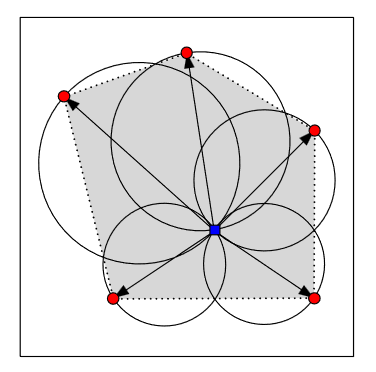
\includegraphics[width=.4\textwidth]{figures/synch/convex_hull.png}
    \caption{Drift vectors comprising the convex hull.\cite{sharfmanGeometricApproachMonitoring2010}}
    \label{fig:convex_hull}
\end{figure}

Each node checks if the ball \( B(e(t), v_i(t)) \) is monochromatic. If a ball is monochromatic red, \( \{x \mid f(x) < r\} \), no communication is
required. If any ball contains green vectors, \( \{y \mid f(y) \geq r\} \), the node reports its local statistics, indicating a local constraint breach.
\Cref{fig:convex_hull} illustrates this concept, showing the drift vectors \( v_i(t) \) for a 2-dimensional statistic on a plane. The convex hull of the drift vectors
is shown in gray, and the union of the balls \( B(e(t), v_i(t)) \) encompasses this convex hull, allowing nodes to collectively monitor the global constraint.

In conclusion, the geometric method presented a substantial breakthrough in monitoring threshold functions over distributed data streams. The findings
of this work provided a pathway for implementing functional monitoring mechanisms, in distributed systems, crucial for the synchronization of Distributed
Learning (DL) processes, and by extension Federated Learning (FL). These mechanisms can substantially reduce the frequency of communication and achieve
efficient learning by applying some simple redefinitions to fit our problem's requirements. Specifically, replacing \emph{nodes} with \emph{clients},
\emph{statistics} with \emph{model parameters}, and providing a fitting \emph{monitor function} of the \emph{local statistics} presents a methodology
directly applicable to the federated setting at hand.

%%%%%%%%%%%%%%%%%%%%%%%%%%%%%%%%%%%%%%%%%%%%%%%%%%%%%%%%%%%%%%%%%%%%%%%%%%%%%%%%%%%%%%%%%%%%%%%%%%%%%%%%%%%%%%%%%%%%%%%%%%%%%%%%%%%%%%%%%%%%%%%%%%%%%%%%%%%%%%
\subsection{Functional Dynamic Averaging}
\subsubsection{The Groundwork:} \label{sec:groundwork}

The encouraging findings of the geometric method\cite{sharfmanGeometricApproachMonitoring2010}, propelled further research leading to
the publication of "Sketch-based Geometric Monitoring of Distributed Stream Queries"\cite{garofalakisSketchbasedGeometricMonitoring2013}
M.Garofalalakis, V.Samoladas and D.Keren with the first two proceeding with "Functional Geometric Monitoring for Distributed Streams"
~\cite{samoladasFunctionalGeometricMonitoring2019}.

Sketch-based Geometric Monitoring\cite{garofalakisSketchbasedGeometricMonitoring2013}
extends the geometric method concept by integrating AMS (Alon-Matias-Szegedy) sketches\cite{alonnogaSpaceComplexityApproximating1996}
with geometric monitoring, enabling efficient and scalable monitoring of complex, non-linear aggregate queries.
This combination allows for significant dimensionality reduction, providing error bounds and approximation guarantees,
and further reducing communication costs, making the method robust against high variability and skew in data streams.

Additionally, the subsequent introduction of Functional Geometric Monitoring (FGM) comprised a conjunction of the
fundamental ideas of geometric monitoring\cite{sharfmanGeometricApproachMonitoring2010} (GM) and the sketches based
approach\cite{garofalakisSketchbasedGeometricMonitoring2013}.

Functional Geometric Monitoring (FGM) employs non-linear functions to project local statistics vectors, or summary vectors, enhancing the flexibility and
performance of monitoring even in scenarios with high data variability and skewness. This approach further reduces communication costs by maintaining
performance within adaptable and strict bounds, closely approximating the coordinator-based version of GM (see \cref{sec:coordinator_based}). FGM also achieves a clear
delineation between monitoring logic and distributed system issues, providing a viable solution for the monitoring logic of any general-purpose middleware
platform. Additionally, FGM introduces the utilization of sketches to approximate local summary vectors and incorporate them into the geometric monitoring
framework, enabling accurate monitoring of complex distributed stream queries.

%%%%%%%%%%%%%%%%%%%%%%%%%%%%%%%%%%%%%%%%%%%%%%%%%%%%%%%%%%%%%%%%%%%%%%%%%%%%%%%
\subsubsection{Methodology:}
\label{sec:methodology}
Building on the promises of previously explored synchronization methods, Functional Dynamic Averaging (FDA) was introduced by V.Konidaris and V.Samoladas
~\cite{konidarisvissarionExtremeScaleOnlineMachine2022} as a sophisticated synchronization strategy for coordinator-based distributed architectures.
FDA presents a compelling approach that can be modified to fit any Distributed or Federated Learning architecture that requires synchronization
as it adopts the characteristic of FGM for separation of the learning process with the undelaying monitoring logic. The application of the
aforementioned approach resulted in substantial mitigation of communication in distributed environments accomplishing not only swift training convergence
but also high levels of accuracy, ranking higher than comparable synchronization methods developed in the same context.

The proposed approach aims to create a global monitoring task that ensures only significant changes in local models are reported,
thereby preserving network bandwidth and reducing latency. Similar to Geometric Monitoring (GM) logic, the objective is to approximate
the global monitoring task by a set of local constraints that can be monitored by all clients. A fundamental principle of Distributed Machine
Learning (DML) is that the global model maintains a good perception of the obtained knowledge, resulting in better performance when it is
closely approximated by the weighted average of all local models. Thus, the proposed constraints must guarantee this initial condition.

The global model is notated as $\bar{w}$ and is generally unknown throughout the learning process. Let $w_t^{(k)}$ be the the model of client $k$ at moment $t$,
then the global model is calculated as follows:
\begin{equation}
    \bar{w} =  \sum_{k=1}^{n} \frac{n_k}{n}w_t^{(i)}
    \label{eq:global_model}
\end{equation}

This indicates, however, that at any given moment $t$ the clients need to be transmitting their model to the server. Such an implementation
would be unreasonable as it would incur particularly frequent communications, deteriorating the performance. Naturally, to address this issue
FDA, similar to other synchronization methods (including BSP, TAP, and SSP), works in rounds, and when the end of a specific round is signaled
then the perceived global model is updated. In other words, at the end of a learning round, all clients send their local models to the server
for aggregation as dictated by \cref{eq:global_model}. The newly-calculated global model is redistributed to the clients providing an estimate of
the global model.

Nonetheless, the question that needs to be answered is how the end of a round is determined. The method of FDA applies a principle that stems
from the FGM approach, utilizing a non-linear projection function to transform the local statistics-summary vectors into real numbers, which are
collectively monitored. In FDA the role of the projection function is assumed by the variance of the local model in comparison with the global estimate.
The reason why variance, is selected is to measure how accurate is the perception we maintain for the global model. In the case that local models start deviating substantially
from the global estimate, this means that a global update is required to bridge this gap, or else the global model's accuracy will deteriorate.

The reason the above is important to answer the question posed is because, in order to identify the end of a round, the value of the variance
needs to surpass a thresholded value $\Theta$. $\Theta$ consists a hyperparameter of FDA that is defined at the start of a training ground and
can be subsequently reconfigured depending on the needs of the synchronization algorithm. The mathematical representation of the above follows:

The global model in notated as $\bar{w}$ and is generally unknown throughout the learning process. Let $w_t^{(k)}$ be the the model of client $k$ at moment $t$,
then the global model is calculated as follows:
\begin{equation}
    \frac{1}{n} \sum_{k=1}^{n} \left\| \mathbf{w}_t^{(k)} - \overline{\mathbf{w}}_t \right\|^2 \leq \Theta
    \label{eq:rtc}
\end{equation}

The condition depicted above is the most crucial part of FDA and is named Round Terminating Condition (RTC) with the left part presenting
model variance and the right the threshold $\Theta$. As long as RTC is not violated it can be induced that the global estimate of the model
is accurate and performs efficiently. That said, FDA introduced three major approaches -Naive FDA, Linear FDA, and Sketch FDA-
differing mainly in how they monitor the Round Termination Condition (RTC) and approximate the variance of the local models.
Each method has a different approach to balancing the trade-off between communication overhead and the accuracy of synchronization.

%%%%%%%%%%%%%%%%%%%%%%%%%%%%%%%%%%%%%%%%%%%%%%%%%%%%%%%%%%%%%%%%%%%%%%%%%%%%%%%
\subsubsection{RTC Monitoring:}
As stated previously in \cref{sec:methodology}, The underlying technique of RTC monitored is entailed by the fundamental principles
of FGM\cite{samoladasFunctionalGeometricMonitoring2019}. In this context, Assume there are $n$ clients in the learning network. Each
of these clients has a local stream generated locally or collected. Let \( S_k(t) \in \mathbb{R}^m \) denote the \emph{local state vector} of client
$k$ in moment $t$. The \emph{global state vector} can be denoted as \( S(t) \in \mathbb{R}^m \) and is computed as the average of all local states.

\begin{equation}
    S(t) = \frac{1}{k}\sum_{i=1}^{k}S_i(t)
    \label{eq:global_state_vector}
\end{equation}

\noindent
The goal is to monitor a bounded condition on the global model, by projecting the global function into real numbers and comparing the projection with threshold $\Theta$.
The projection function is non-linear and is denoted as $F :\mathbb{R}^m \rightarrow \mathbb{R}$ leading to the following condition:
\begin{equation}
    \label{eq:objective}
    F(S(t)) \leq \Theta \xRightarrow{\ref{eq:global_state_vector}} F(\frac{1}{k}\sum_{i=1}^{k}S_i(t)) \leq \Theta
\end{equation}

\noindent
Additionally, let \( t_0 \) be the time when the latest communication round started. At this initial time, the local models are synchronized,
so \( w_{t_0}^{(1)} = w_{t_0}^{(2)} = \cdots = w_{t_0}^{(n)} = \bar{w}_{t_0} \). The \emph{update of learner} \( k \) at step \( t \)
is the difference between the weights at step \( t \) and the weights at the last synchronization \( t_0 \) which represents the
estimation of the global state. Thus the average update can also be induced as the mean of the clients' updates. Overall:

\begin{equation}
    \label{eq:learner_update}
    \begin{cases}
        \Delta_t^{(k)} = w_t^{(k)} - w_{t_0}^{(k)} \text{: Update of learner \( k \) at step \( t \)} \\
        \bar{\Delta}_t = \frac{1}{n} \sum_{k=1}^{n} \Delta_t^{(k)} \text{: Average update}
    \end{cases}
\end{equation}

\noindent
With these definitions in mind we can proceed and reformulate the norm calculation on the left side of RTC \cref{eq:rtc}:\

\begin{align}
    \frac{1}{n} \sum_{k=1}^{n} \left\| w_t^{(k)} - \bar{w}_t \right\|^2
     & = \frac{1}{n} \sum_{k=1}^{n} \left\| \left(w_t^{(k)} - w_{t_0}^{(k)}\right) - \left( \bar{w}_t - w_{t_0}^{(k)} \right) \right\|^2 \notag                                                                   \\
     & = \frac{1}{n} \sum_{k=1}^{n} \left\| \Delta_t^{(k)} - \bar{\Delta}_t \right\|^2 \notag                                                                                                                     \\
     & = \frac{1}{n} \sum_{k=1}^{n} \left( \left\| \Delta_t^{(k)} \right\|^2 - 2 \Delta_t^{(k)} \cdot \bar{\Delta}_t + \left\| \bar{\Delta}_t \right\|^2 \right) \notag                                           \\
     & = \left( \frac{1}{n} \sum_{k=1}^{n} \left\| \Delta_t^{(k)} \right\|^2 \right) - 2 \left( \frac{1}{n} \sum_{k=1}^{n} \Delta_t^{(k)} \right) \cdot \bar{\Delta}_t + \left\| \bar{\Delta}_t \right\|^2 \notag \\
     & = \left( \frac{1}{n} \sum_{k=1}^{n} \left\| \Delta_t^{(k)} \right\|^2 \right) - \left\| \bar{\Delta}_t \right\|^2
    \label{eq:variance_calc}
\end{align}

\noindent
Thus, conceptually we can set the local state of client $k$ and the function $F$ in the following manner to satisfy our objective\cref{eq:objective}:

\begin{equation}
    \label{eq:local_state_and_function}
    \begin{cases}
        S_k(t) = \left[ \| \Delta_t^{(k)} \|^2, \Delta_t^{(k)} \right]^T \in \mathbb{R}^{m+1}, \\
        F\left( \left[ v, x \right]^T \right) = v - \| x \|^2
    \end{cases}
\end{equation}
\noindent
Using these aforementioned definitions, the RTC can be expressed as:
\[
    F(S(t)) \leq \Theta,
\]

%%%%%%%%%%%%%%%%%%%%%%%%%%%%%%%%%%%%%%%%%%%%%%%%%%%%%%%%%%%%%%%%%%%%%%%%%%%%%%%
\subsubsection{Practical Considerations}

Defining the local state \( S_k(t) \) in the described manner in \cref{eq:local_state_and_function} can be resource-intensive for the network, as
the local update \( \Delta_t^{(k)} \)
has \( m \) dimensions, corresponding to the number of weights in the local client’s model. Therefore, our goal is to examine different ways to
define the local states and the function \( F \) to minimize network overhead. This process leads to the presentation of the three proposed FDA
approaches, each opting for a different approach of dimensionality reduction on the local updates $\Delta^{(i)}$. The idea is that as the
approximation of the actual RTC becomes stricter, the cost of communication increases. This trade-off is inevitable and will be studied further,
with the three methods being presented with increasing communication cost, yet decreasing approximation accuracy.

%%%%%%%%%%%%%%%%%%%%%%%%%%%%%%%%%%%%%%%%%%%%%%%%%%%%%%%%%%%%%%%%%%%%%%%%%%%%%%%
Nonetheless, at this point, the
general algorithmic approach of FDA is attached to maintain a common offset before the upcoming branching in the three approaches. The
following algorithm is a product of M. Theologitis thesis-dissertation\cite{theologitismichaelAlgorithmsOnlineFederated2023}.

\begin{algorithm}[H]
    \caption{FDA: FL training with Approximate RTC Monitoring}
    \begin{algorithmic}
        \Require $f(w)$: Stochastic objective function with parameters $w \in \mathbb{R}^d$
        \Require $K$: The number of clients indexed by $k$
        \Require $\Theta$: Monitoring threshold
        \Require $S_k(t)$: The local state for client $k$ where $S_k(t) \in \mathbb{R}^p$ and $p \ll d$
        \Require $F(x)$: A function $F : \mathbb{R}^p \to \mathbb{R}$ such that $F(S(t)) \leq \Theta$ implies the RTC
        \Require $\eta$: Step size (learning rate)
        \Require $s$: The number of local steps
        \Require $b$: The local mini-batch size
        \State \textbf{Server executes:}
        \Indent
        \State initialize $w_1$
        \For{each round $t = 1, 2, \ldots$}
        \State Broadcast $w_t$ to all clients
        \Repeat
        \For{each client $k = 1, \ldots, K$ \textbf{in parallel}}
        \State $S_k(t) \leftarrow \text{ClientTrain}(k)$
        \EndFor
        \Until{$F(S(t)) > \Theta$}
        \For{each client $k = 1, \ldots, K$ \textbf{in parallel}}
        \State $w_{t+1}^{(k)} \leftarrow$ (download the model of client $k$)
        \EndFor
        \State $w_{t+1} \leftarrow \sum_{k=1}^{K} \frac{n_k}{n} w_{t+1}^{(k)}$
        \EndFor
        \EndIndent

        \State \textbf{ClientTrain}$(k)$:
        \Indent
        \State $\mathcal{B} \leftarrow$ (Choose $s$ batches of size $b$ from $\mathcal{P}_k$)
        \For{each batch $B \in \mathcal{B}$}
        \State $w \leftarrow w - \eta \nabla f_B(w)$
        \EndFor
        \State return $S_k(t)$ to server
        \EndIndent
    \end{algorithmic}
\end{algorithm}

%%%%%%%%%%%%%%%%%%%%%%%%%%%%%%%%%%%%%%%%%%%%%%%%%%%%%%%%%%%%%%%%%%%%%%%%%%%%%%%
\subsubsection{Naive Approximation}
The Naive FDA unlike Naive, which ignores the local state vector, simplifies the problem by reducing the local state to a single scalar value,
specifically the squared norm of the local update vector. This approach is straightforward and incurs minimal computation overhead, making it
suitable for scenarios where communication costs are critical. The local state for client $k$ at time $t$, along with the projection function
$F$ are reformed:

\begin{equation}
    \begin{cases}
        S_k(t) = \|\Delta_t^{(k)}\|_2^2 \\
        F\left(v\right) = v
    \end{cases}
    \label{eq:naive}
\end{equation}

\noindent
The function $F(v) = v$ is used to aggregate the states across clients. The RTC is checked using the condition $F(S(t)) \leq \Theta$.
The proof that Naive FDA satisfies the RTC involves starting from the condition we want to prove and with logical equalities
conclude in a known condition (RTC):

\begin{align}
    F(S(t)) \leq \Theta & \iff \frac{1}{n}\sum_{k=1}^{n} \left\|\Delta_{t}^{(k)}\right\|^2 \leq \Theta \notag                                                                                                                                                                     \\
                        & \overset{\left\| \overline{\Delta}_t \right\|^2 \geq 0}{\iff} \frac{1}{n} \sum_{k=1}^{n} \left\|\Delta_{t}^{(k)}\right\|^2 - \left\| \overline{\Delta}_t \right\|^2 \leq \frac{1}{n}\sum_{k=1}^{n} \left\|\Delta_{t}^{(k)}\right\|^2 \leq \Theta \notag \\
                        & \overset{\ref{eq:variance_calc}}{\iff} \frac{1}{n}\sum_{k=1}^{n} \left\| \mathbf{w}_t^{(k)} - \overline{\mathbf{w}}_t \right\|^2 \leq \frac{1}{n}\sum_{k=1}^{n} \left\|\Delta_{t}^{(k)}\right\|^2 \leq \Theta \notag                                    \\
                        & \implies \frac{1}{n}\sum_{k=1}^{n} \left\| \mathbf{w}_t^{(k)} - \overline{\mathbf{w}}_t \right\|^2 \leq \Theta \quad \text{\underline{RTC}} \quad (\Cref{eq:rtc})
\end{align}

\noindent
Since this aggregation overestimates the actual variance, ensuring $F(S(t)) \leq \Theta$ implies that the RTC is met.
This approach is the most simple requiring merely a 1-dimensional scalar value to be communicated to monitor RTC.\ In most cases, accuracy
is not heavily impacted, yet this approximation is based on a loose condition, meaning that deviation from the required
results can be noticed in some cases.

%%%%%%%%%%%%%%%%%%%%%%%%%%%%%%%%%%%%%%%%%%%%%%%%%%%%%%%%%%%%%%%%%%%%%%%%%%%%%%%
\subsection{Linear Approximation}
The Linear FDA method provides a more refined approach by reducing the local update vector $\Delta_t^{(k)}$ to a scalar product with a unit vector $\xi$, meaning
$\xi \cdot \Delta_t^{(k)} \in \mathbb{R}$.
This method balances computational efficiency and accuracy in estimating the variance of the updates. The local state for
client $k$ at time $t$, along with the projection function $F$, are defined as:

\begin{equation}
    \begin{cases}
        S_k(t) = \left[|\Delta_t^{(k)}|_2^2, \langle \xi, \Delta_t^{(k)} \rangle\right]^\top \\
        F(v, x) = v - x^2
    \end{cases}
    \label{eq:linear_redefinition}
\end{equation}

\noindent
The function $F(v, x) = v - x^2$ is used to aggregate the states across clients. The RTC is checked using the condition $F(S(t)) \leq \Theta$.
The proof that Linear FDA satisfies the RTC follows the same methodology as in Naive:

\begin{align}
    F(S(t)) \leq \Theta & \iff \frac{1}{n} \sum_{k=1}^{n} \left\| \Delta_{t}^{(k)} \right\|^2 - \frac{1}{n} \sum_{k=1}^{n} (\xi \cdot \Delta_{t}^{(k)})^2 \leq \Theta \notag                                                                                                                 \\
                        & \overset{\xi^2 = 1}{\iff} \frac{1}{n} \sum_{k=1}^{n} \left\| \Delta_{t}^{(k)} \right\|^2 - \left\| \overline{\Delta}_{t} \right\|^2 \leq \frac{1}{n} \sum_{k=1}^{n} \left\| \Delta_{t}^{(k)} \right\|^2 - (\xi \cdot \overline{\Delta}_{t})^2 \leq \Theta \notag   \\
                        & \overset{\ref{eq:variance_calc}}{\iff} \frac{1}{n} \sum_{k=1}^{n} \left\| \mathbf{w}_{t}^{(k)} - \overline{\mathbf{w}}_{t} \right\|^2 \leq \frac{1}{n} \sum_{k=1}^{n} \left\| \Delta_{t}^{(k)} \right\|^2 - (\xi \cdot \overline{\Delta}_{t})^2 \leq \Theta \notag \\
                        & \implies \frac{1}{n} \sum_{k=1}^{n} \left\| \mathbf{w}_{t}^{(k)} - \overline{\mathbf{w}}_{t} \right\|^2 \leq \Theta \quad \text{RTC (\Cref{eq:rtc})}
\end{align}
\noindent
This method ensures that the variance is accurately estimated, and the condition $F(S(t)) \leq \Theta$ implies the RTC is met.
This approach balances communication efficiency and accuracy, making it suitable for scenarios requiring a more precise
estimate than the Naive method. A key consideration, nonetheless for this approach is the selection of $\xi$. A random selection of $\xi$
is likely to perform inadequately (leading to early termination of a round), as it may be nearly orthogonal to $\Delta$. A preferable
choice would be a vector that is correlated with $\Delta$. One heuristic option is to use $\Delta_0$ (normalized to have a unit norm),
which is the update vector from right before the current round commenced. Each node can estimate this independently without needing
communication, as it is the difference between the last two models, $\tilde{w}_0 - \tilde{w}_1$, sent by the coordinator.
%%%%%%%%%%%%%%%%%%%%%%%%%%%%%%%%%%%%%%%%%%%%%%%%%%%%%%%%%%%%%%%%%%%%%%%%%%%%%%%

\subsection{Sketch FDA}
The Sketch FDA method utilizes AMS sketches\cite{garofalakisSketchbasedGeometricMonitoring2013} to compress local update vectors, achieving an optimal
balance between communication efficiency and accuracy. This technique is particularly advantageous in scenarios involving high-dimensional data that require
significant dimensionality reduction. The underlying logic and analysis presented here follow the methodology outlined by Frangias\cite{frangiasgeorgiosFederatedLearningTensorFlow2023}
in his comprehensive study on FDA.

The AMS sketch denoted as \( \text{sk}( \mathbf{v} ) \), is a technique that compresses
a high-dimensional vector into a significantly smaller matrix. For a vector \( \mathbf{v} \in \mathbb{R}^M \), the sketch \( \text{sk}( \mathbf{v} ) \)
is defined as:

\begin{equation}
    \text{sk}( \mathbf{v} ) = \Xi = [ \xi_1 \quad \xi_2 \quad \ldots \quad \xi_d ],
    \label{eq:sketch_definition}
\end{equation}

\noindent
where each \( \xi_i \) is a sub-vector of dimension \( d \), and typically \( d \cdot m \ll M \).

% \noindent
The sketch function is linear and can be computed in \( O(dM) \) steps. Furthermore, there exists a function, denoted as \( \mathcal{M}_2 \), that accurately
estimates the squared norm of a vector \( \mathbf{v} \) using its sketch \( \text{sk}( \mathbf{v} ) \). This function is defined as:

\begin{equation}
    \mathcal{M}_2(\text{sk}(\mathbf{v})) = \text{median}_{i=1,\ldots,d} \| \xi_i \|^2.
    \label{eq:squared_norm_estimate}
\end{equation}

\noindent
For \( m = O \left( \frac{1}{\epsilon^2} \right) \) and \( d = O \left( \log \frac{1}{\delta} \right) \), it is proven that with high probability (\( 1 - \delta \)),
the squared norm \( \| \mathbf{v} \|^2 \) can be approximated within a factor of \( (1 - \epsilon) \) to \( (1 + \epsilon) \):

\begin{equation}
    (1 - \epsilon) \| \mathbf{v} \|^2 \leq \mathcal{M}_2(\text{sk}(\mathbf{v})) \leq (1 + \epsilon) \| \mathbf{v} \|^2.
    \label{eq:approximation}
\end{equation}

\noindent
In our context, the large vector requiring compression is the local update \( \Delta_t^{(k)} \in \mathbb{R}^M \). Consequently, the local state \( S_k(t) \) and the function
\( F \) for the sketch method are defined as follows:

\begin{equation}
    \begin{cases}
        S_k(t) = \left[ \left\| \Delta_t^{(k)} \right\|^2 \quad \text{sk} \left( \Delta_t^{(k)} \right) \right]^T \in \mathbb{R}^{1 + d \times m}, \\
        F \left( \begin{array}{c} v \\ \Xi \end{array} \right) = v - \frac{1}{1 + \epsilon} \mathcal{M}_2(\Xi).
    \end{cases}
    \label{eq:sketch_redefinition}
\end{equation}


\noindent
To establish that the RTC holds, we proceed as follows:

\begin{align}
    F(S(t)) \leq \Theta & \iff \frac{1}{n} \sum_{k=1}^n \left\| \Delta_t^{(k)} \right\|^2 - \frac{1}{1 + \epsilon} \cdot \frac{1}{n} \sum_{k=1}^n \mathcal{M}_2 \left( \text{sk} \left( \Delta_t^{(k)} \right) \right) \leq \Theta \notag                                                                                                       \\
                        & \overset{\text{linearity}}{\iff} \frac{1}{n} \sum_{k=1}^n \left\| \Delta_t^{(k)} \right\|^2 - \frac{1}{1 + \epsilon} \cdot \mathcal{M}_2 \left( \text{sk} \left( \Delta_t \right) \right) \leq \Theta \notag                                                                                                          \\
                        & \overset{\ref{eq:approximation}}{\iff} \frac{1}{n} \sum_{k=1}^n \left\| \Delta_t^{(k)} \right\|^2 - \left\| \overline{\Delta}_t \right\|^2 \leq \frac{1}{n} \sum_{k=1}^n \left\| \Delta_t^{(k)} \right\|^2 - \frac{1}{1 + \epsilon} \mathcal{M}_2 \left( \text{sk} \left( \Delta_t \right) \right) \leq \Theta \notag \\
                        & \overset{\ref{eq:variance_calc}}{\implies} \frac{1}{n} \sum_{k=1}^n \left\| \mathbf{w}_t^{(k)} - \overline{\mathbf{w}}_t \right\|^2 \leq \Theta \quad \text{\underline{RTC} (\Cref{eq:rtc})}
\end{align}

%%%%%%%%%%%%%%%%%%%%%%%%%%%%%%%%%%%%%%%%%%%%%%%%%%%%%%%%%%%%%%%%%%%%%%%%%%%%%%%%%%%%%%%%%%%%%%%%%%%%%%%%%%%%%%%%%%%%%%%%%%%%%%%%%%%%%%%%%%%%%%%%%%%%%%%%%%%%%%
\subsection{Multiprogramming \& Synchronization Primitives in DML}
Learning in Distributed Machine Learning Systems is a complicated process that involves one or more servers that orchestrate
and manage a great number of worker nodes. Especially if we consider the applicability of FL in the Internet of Things (IoT)
scenarios, the number of coordinated nodes can be humongous. For this reason, a plethora of synchronization mechanisms
need to be employed on the server side to ensure that updates to the model parameters are consistent and free from conflicts.
Multiprogramming and synchronization primitives play a crucial role in achieving this goal by managing access to shared resources and preventing race conditions. The purpose of this section is to highlight the principal mechanisms utilized in this context providing
a comprehensive overview.

\paragraph{Locks}
are fundamental in distributed machine learning for protecting shared resources such as model parameters, ensuring that only
one node can modify these resources at a time. Locks help prevent data corruption by enforcing mutual exclusion. However, they can
lead to high contention and potential deadlocks. Techniques like lock striping and sharding are used to reduce contention by breaking
down large locks into smaller, more manageable parts, allowing greater parallelism and reducing the likelihood of performance bottlenecks

\paragraph{Mutexes (mutual exclusions)}
provide a robust mechanism for ensuring exclusive access to critical sections of code, particularly when updating shared model parameters. 
They prevent multiple nodes from making concurrent updates that could lead to inconsistent states. Challenges include avoiding priority 
inversion, where a high-priority task is blocked by a lower-priority one. Priority inheritance protocols are employed to temporarily elevate 
the priority of the task holding the mutex, mitigating this issue.

\paragraph{Semaphores}
manage access to limited resources such as GPUs in distributed machine learning. By controlling the number of concurrent accesses, 
they ensure efficient and fair resource utilization. Semaphores prevent resource exhaustion with timeout 
mechanisms that allow tasks to fail gracefully if they cannot acquire a semaphore within a specified time. Proper exception handling ensures 
semaphores are released correctly, preventing resource leaks and maintaining system stability.

\paragraph{Condition Variables}
synchronize nodes based on specific conditions or events, allowing threads to wait until certain conditions are met. This 
is crucial in distributed machine learning for coordinating updates and ensuring that nodes do not proceed until necessary conditions are satisfied. 
Condition variables must handle challenges like missed signals and spurious wakeups. Robust signaling mechanisms, combined with atomic variables, 
ensure that condition checks are reliable and that threads are correctly awakened only when the desired conditions are truly met.\

\paragraph{Read-Write Locks:}
Read-write locks are particularly useful in scenarios where model parameters are read frequently but updated infrequently. They allow multiple nodes 
to read data simultaneously while ensuring exclusive access for write operations. This improves efficiency and maintains consistency in model states. 
Read-write locks must address writer starvation, which occurs when writers are perpetually blocked by continuous read operations. Fairness policies 
that prioritize writers after a certain number of reads help mitigate this issue, ensuring balanced access to resources.

\subsubsection{Ensuring Model Consistency:}
Ensuring model consistency in distributed machine learning involves carefully designing synchronization mechanisms to prevent data corruption and
ensure coherent updates. In this context, multiprogramming and synchronization primitives are essential for maintaining model consistency and ensuring
efficient resource utilization. By leveraging locks, mutexes, semaphores, condition variables, and read-write locks, server-side systems can synchronize updates,
prevent race conditions, and manage access to shared resources effectively. Understanding and correctly implementing these primitives is crucial for building
robust and high-performance distributed machine learning systems. Key considerations to achieve the above include:

\begin{enumerate}
    \item \emph{Avoiding Deadlocks:} In a distributed setting, deadlocks can occur when multiple nodes wait indefinitely for resources held by each
          other. Techniques such as establishing a strict order for acquiring locks and implementing timeout mechanisms can help
          avoid deadlocks.
    \item \emph{Minimizing Lock Contention:} Lock contention arises when multiple nodes attempt to acquire the same lock, leading to delays. Reducing
          the granularity of locks and minimizing the duration of critical sections can help alleviate lock contention.
    \item \emph{Preventing Priority Inversion:} Priority inversion occurs when a high-priority node is blocked by a lower-priority node holding a lock.
          Implementing priority inheritance protocols can mitigate this issue by temporarily elevating the priority of the
          lower-priority node.
    \item \emph{Efficient Barrier Synchronization:} Barrier synchronization ensures that all nodes reach a certain point in computation before proceeding.
          This is critical in distributed training phases, ensuring that all nodes have completed their updates before the next iteration begins.
\end{enumerate}

%%%%%%%%%%%%%%%%%%%%%%%%%%%%%%%%%%%%%%%%%%%%%%%%%%%%%%%%%%%%%%%%%%%%%%%%%%%%%%%%%%%%%%%%%%%%%%%%%%%%%%%%%%%%%%%%%%%%%%%%%%%%%%%%%%%%%%%%%%%%%%%%%%%%%%%%%%%%%%